% !TEX root = ../Dokumentation.tex
\section{Technologierecherche}
\subsection{Funktionsweise der Hardware}
Für die geplante Arbeit wird ein Raspberry Pi 3, eine 32GB SD-Karte, eine Basisplatine, Sensorplatinen mit Temperaturfühlern sowie entsprechende Verbindungskabel verwendet. Das Raspberry Pi ist ein Einplatinencomputer und eignet sich mit seinen Funktionen und Komponenten besonders gut für diese Arbeit. Über die elektrischen Anschlusspunkte, auch GPIOs genannt, werden die Messsignale des Temperatursensors abgefragt. Mittels der Basisplatine, welche an das Raspberry angeschlossen wird, können die gelieferten Daten der angeschlossenen Sensoren von einem analogen zu einem digitalen Signalen umgewandelt werden.
Diese digitalen Signale können so in Temperaturwerte umgerechnet und für eine kontinuierliche Anzeige bereitgestellt werden.

\begin{figure}[H]%Position festigen
\centering
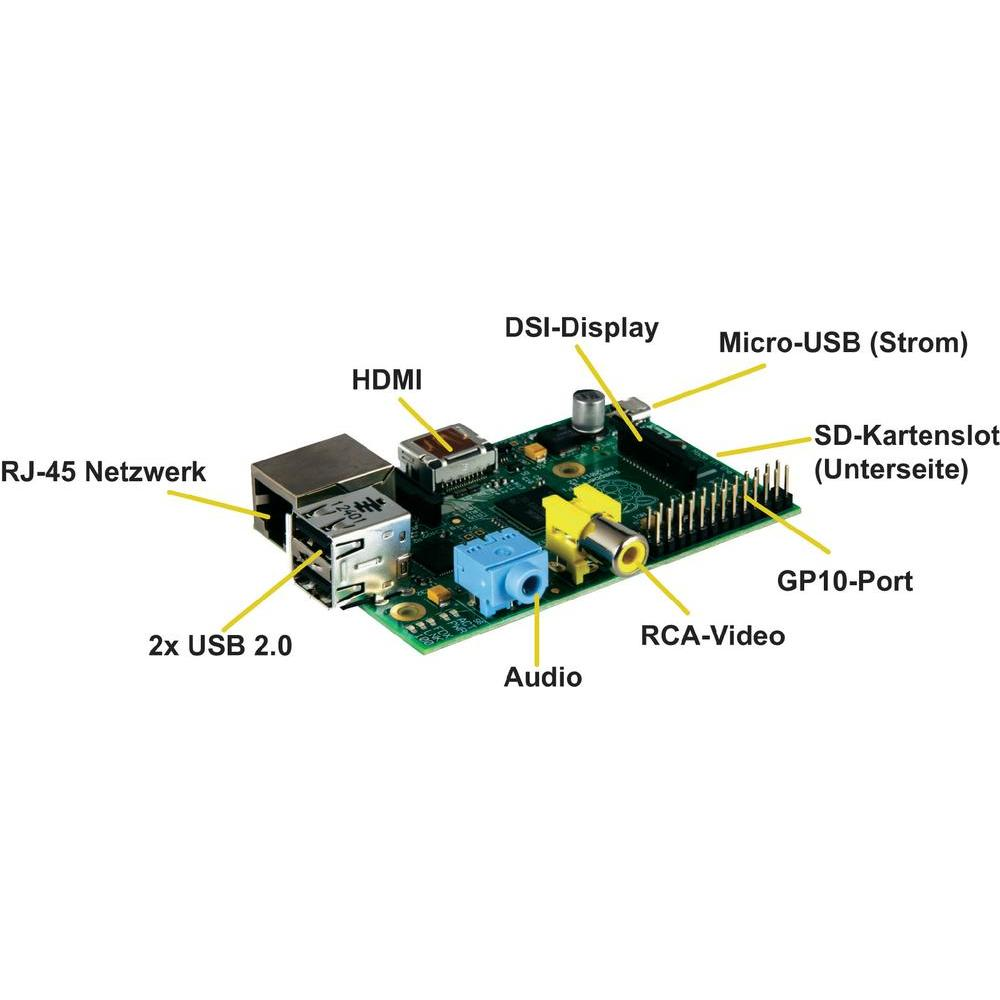
\includegraphics[width=1\textwidth]{Images/RaspberryPi.jpg}
\caption{Pi (Quelle www.Conrad.ch)}
\label{fig:raspi}
\end{figure}

\subsubsection{GPIO}
GPIO ist ein elektrischer Anschlusspunkt, welcher vom RaspberryPi zur Verfügung gestellt wird. Über diese Schnittstelle können die Werte der anschlossenen Sensoren übertragen werden.

\subsection{Software Entwurfsmuster}